\documentclass[journal]{IEEEtran}
\usepackage{graphicx}
\usepackage{subfigure}
\usepackage{url}
\ifCLASSINFOpdf
\else
\usepackage[dvips]{graphicx}
\fi
\usepackage{url}

\hyphenation{op-tical net-works semi-conduc-tor}

\usepackage{mathtools}
\DeclarePairedDelimiter\ceil{\lceil}{\rceil}
\DeclarePairedDelimiter\floor{\lfloor}{\rfloor}

\usepackage{graphicx}


\begin{document}
	
	\title{ Time-series classification using matrix-based methods: Application to blackhole state identification of RXTE satellite data}
	
	\author{First A. Author, \IEEEmembership{Fellow, IEEE}, Second B. Author, and Third C. Author, Jr., \IEEEmembership{Member, IEEE}
		\thanks{This paragraph of the first footnote will contain the date on which you submitted your paper for review. It will also contain support information, including sponsor and financial support acknowledgment. For example, ``This work was supported in part by the U.S. Department of Commerce under Grant BS123456.'' }
		\thanks{The next few paragraphs should contain the authors' current affiliations, including current address and e-mail. For example, F. A. Author is with the National Institute of Standards and Technology, Boulder, CO 80305 USA (e-mail: author@boulder.nist.gov).}
		\thanks{S. B. Author, Jr., was with Rice University, Houston, TX 77005 USA. He is now with the Department of Physics, Colorado State University, Fort Collins, CO 80523 USA (e-mail: author@lamar.colostate.edu).}}
	
	\markboth{Journal of \LaTeX\ Class Files, Vol. 14, No. 8, August 2015}
	{Shell \MakeLowercase{\textit{et al.}}: Bare Demo of IEEEtran.cls for IEEE Journals}
	\maketitle
	
	\begin{abstract}
		Across diverse domains such as medicine, weather, finance, agriculture, astronomy, etc., it is required to deal with timeseries of measurements. Classification of timeseries as stochastic (noise-like) or non-stochastic (which has a well-defined structure), helps understand the underlying phenomenon. The methods used to accomplish this classification are either : (i) Correlation Integral (CI)-based or (ii) Entropy-based approaches, both of which are computationally expensive. In this work, we propose two matrix-based methods to achieve stochastic vs non-stochastic classification, without requiring the computation-intensive phase space. The proposed matrix-based methods are: (a) SVD-decomposition followed by topological analysis (using Betti number descriptors) (b) PCA-based technique. The proposed methods have been applied to synthetic data, as proof of concept. The utility of the methods is illustrated on astronomy data which are 12 categories of timeseries pertaining to blackhole \textit{GRS 1915 + 105}, obtained from RXTE satellite. Comparisons of obtained results with those in literature are also presented. The order of computational complexity using the proposed approaches is XXXXXXX of N, where N is the length of the timeseries. In contrast, CI based approaches require XXXX, while Entropy-based approaches need XXXXX. It is found that among the proposed matrix based methods, SVD analysis concurs with CI based analysis on all 12 categories of time series utilized. However, the inference using PCA based approach illustrates that one class among the 12 turns out to be inconsistent with the other approaches. Investigation into these (in)consistencies  is expected to have long standing implications in astrophysics and otherwise.
		
		
		
		%Black hole is one of the fascinating,  however mysterious, astrophysical  objects. In order to identify it one has to look at its environment, often forming a disc-like structure. This disc, called accretion disc, evolves with time transiting from one state to another. For example, in one extreme regime it shows temperature dependent radiations making the disc geometrically thin, and in yet another extreme  regime of time span however radiation turns out to be temperature independent making the disc hot and geometrically thick.  Nevertheless, in general, accretion disc lies in  states intermediate between the two extremes. The present mission is to capture black hole states  explicitly using SVD and PCA based decompositions. In order to do that we rely on time series data of black hole \textit{GRS 1915 + 105} obtained from RXTE satellite. As a black hole cannot be seen directly, identifying its states accurately could help in characterizing its properties. Earlier time series  analysis based on Correlation Integral (CI) approaches, supplemented by theory, argued for four specific states. However there are caveats when data themselves are not free from noise and the  appropriate method for such an analysis itself is exploratory. Present interdisciplinary study aims at, on one hand,  to cross-verify the previous inference, on the other hand to identify, if any,  novel characteristics of black holes. In the experiments conducted it is found that among the proposed matrix based methods, SVD analysis concurs with CI based analysis on all the 12 classes of time series utilized. However, the inference using PCA based approach illustrates that one  class among the 12 turns out to be inconsistent with the other approaches. Investigation into these (in)consistencies  is expected to have long standing implications in astrophysics and otherwise.
	\end{abstract}
	
	\begin{IEEEkeywords}
		Timeseries classification, stochastic, non-stochastic, SVD analysis, PCA analysis %\url{http://www.ieee.org/organizations/pubs/ani_prod/keywrd98.txt}
	\end{IEEEkeywords}
	
	
	\IEEEpeerreviewmaketitle
	
	
	
	\section{Introduction}
	Several real-world phenomena are studied by collecting associated measurements over time, popularly called as timeseries. Timeseries classification as stochastic (noise-like) or non-stochastic (which has a well-defined structure), is the first step in understanding the underlying physical phenomenon. Standard stochastic signals such as white noise, pink noise, etc. exhibit characteistics such as nearly zero auto-correlation coefficients for all possible values of lags and a power spectral density that decays with frequency. The rate of decay determines the kind of noise. On the other hand, standard non-stochastic signals such as Logistic map (at growth rate = 4), Lorenz system result in timeseries that exhibit a well-defined structure, such as having a certain number of fixed points. For such phenomena, computing parameters such as Correlation Dimension helps in revealing the underlying dynamics. However, for stochastic timeseries the Correlation Dimension never saturates. Hence if the goal of the study is to check if the timeseries is stochastic, then such computations must be avoided. 
	
	
	In literature, methods that accomplish this classification can be broadly categorised as : (i) Correlation Integral based (ii) Entropy-based. Correlation Integral based approach was proposed in \cite{CIGRacia}. It is a computation-intensive process, since the Correlation Integral (CI) needs to be computed for different choices of Embedding dimension, which can only be approximated using the autocorrelation plot. Besides, it is well-known that this value of correlation dimension does not saturate for a stochastic time series. Hence to establish if the considered timeseries is stochastic, this computation needs to be repeated for a large range of values of Embedding Dimension, making the order of computations needed greater by that factor. Entropy-based approaches \cite{baretto, russian, splrecent} utilize concepts of phase-space. This is also a computation-intensive process, with several assumptions about the phenomenon that resulted in the timeseries. TODO write something more on ENtropy based methods.
	
	The problem of stochastic vs non-stochastic classification is important for one of the challenging problems in astrophysics, which could lead to the understanding of black holes. As a black hole cannot be seen directly, to identify it, one has to look for its environment forming a disc-like structure by the infalling matter called accretion disc. In this work, we focus on the black hole source \textit{GRS 1915+105}, which presents several intriguing facets. It has been divided into 12 different temporal categories: $\alpha$, $\beta$, $\gamma$, $\delta$, $\lambda$, $\kappa$, $\mu$, $\nu$, $\rho$, $\phi$, $\chi$ and $\theta$ \cite{Belloni2000}, with their respective distinct timeseries. One fundamental aspect of the understanding is to determine if the black hole source is stochastic or non-stochastic (implying turbulent nature of the system). There are studies reported that utilize the Correlation Integral (CI) approach to determine the characterization of this specific black hole data \cite{Mukhopadhyay2004, misra2006}. However, in this work, we propose to utilize matrix-based methods, Principal Component Analysis (PCA) and Singular Value Decomposition (SVD), to understand the same data. It is useful to compare the inferences obtained using these distinct approaches; the implications of the (dis)similarities in inferences, if any, could lead to better understanding of the temporal dynamics of the system.
	
	It is widely known that the true nature of the source is understood by studying both temporal and spectral features. If the source radiation is temperature dependent, it is called multicolour blackbody or ``diskbb" \cite{Shakura1973}. On the other hand, the temperature independent radiation consists of power-law tail (``PL") \cite{chakrabarti1995,narayan1994}. The difference in their implications lies in the fact that the former leads the underlying accretion disc around the black hole to be geometrically thin, while the latter leads to a geometrically thick disc. Studies in literature combine these observations into four possible black hole states \cite{Adegoke2018}:
	\begin{enumerate}
		\item Non-stochastic and diskbb: Keplerian disc \cite{Shakura1973}.
		\item Non-stochastic and PL: Advection Dominated Accretion Flow (ADAF)  \cite{narayan1994}.
		\item Stochastic and diskbb: Slim disc \cite{Abramowicz1988}.
		\item Stochastic and PL: General Advective Accretion Flow (GAAF) \cite{chakrabarti1995, rajesh2010}.
	\end{enumerate}
	
	
%	Interestingly, to quantify the properties of a black hole source, along with temporal features one has to look for spectral features as well, they together lead to the true nature of the source. If the source radiation is temperature dependent, it produces more like a blackbody radiation, namely multicolour blackbody or ``diskbb" \cite{Shakura1973}. On the other hand, the temperature independent radiation consists of a power-law tail, named as ``PL" \cite{chakrabarti1995,narayan1994}. While the former leads the underlying accretion disc around the black hole to be geometrically thin, the latter leads to a geometrically thick disc.
%	
%	In the present study, black hole states are determined by  classifying the given time series, which is photon count rate as a function of time,  as being either stochastic or non-stochastic. This classification is performed using classical matrix based methods, SVD and PCA.
%	However, the novelty of the study lies in (i) quantifying temporal complexity obtained by SVD decomposition, using topological techniques and (ii) utilizing features derived from PCA for classification. Based on our analysis there are four possible black hole states \cite{Adegoke2018}:
%	\begin{enumerate}
%		\item Non-stochastic and diskbb: Keplerian disc \cite{Shakura1973}.
%		\item Non-stochastic and PL: Advection Dominated Accretion Flow (ADAF)  \cite{narayan1994}.
%		\item Stochastic and diskbb: Slim disc \cite{Abramowicz1988}.
%		\item Stochastic and PL: General Advective Accretion Flow (GAAF) \cite{chakrabarti1995, rajesh2010}.
%	\end{enumerate}
	 The contributions of this paper:
	\begin{itemize}
		\item SVD decomposition of the data matrix is used for identifying temporal dynamics of the time series as in \cite{misra2006}. The novelty in the work is that this decomposition is followed by topological analysis of the plot involving the top two right singular vectors for classification of a time series as stochastic or non-stochastic. 
		
		\item PCA, which is widely used approach for decorrelating features and dimensionality reduction, is utilized to classify a time series as stochastic vs non-stochastic. We propose a novel approach that hierarchically splits the timeseries, computing eigenvalue ratios of covariance matrix of data sub-intervals, exhaustively. Multiple features are devised from the eigenvalue ratios, which are utilized as input features to a linear SVM for classification as stochastic or non-stochastic.
	\end{itemize}
	
	
	\section{Related Work}
	Several groups have worked on distinguishing between stochastic and non-stochastic time series. The idea of utilizing Permutation Entropy (PE) to determine the complexity measure of a time series was explored in \cite{Bandt2002}. In the work reported in \cite{Boaretto2021}, PE was used to parameterize a given time series  followed by classification using  Neural Network. The paper explored the idea of utilizing PE of a time series to determine if it is strongly correlated with known stochastic signals (noise).   The claim was that for non-stochastic signals the deviation of the parameter is relatively large as compared to that of the parameter of a stochastic signal. Another set of reported studies are based on  graph theory. In the work reported in \cite{lacasa2010}, the authors have utilized the horizontal visibility algorithm in order to distinguish between stochastic and non-stochastic processes. A recent work, reported in \cite{Silva2022}, mapped time series into  graphs and computed various topological properties, which they called \textit{NetF}, capturing  measures such as centrality, distance, connectivity etc. PCA was applied on the \textit{NetF} feature matrix and clustering was performed on the principal components.
	
	In the approach outlined in \cite{Brunton2016}, the authors combined the idea of sparsity and machine learning with non-linear dynamical systems, in order to determine the governing dynamics. Sparse regression was used to determine the fewest terms in the equations that govern the dynamics of the phenomenon. The user-defined dictionary of basis functions consists of well-known functions such as polynomials, trigonometric functions and exponentials. However, the optimal choice of dictionary for a specific choice of problem remains a challenge.
	
	In this work, we propose to utilize classical matrix based methods which do not require any assumptions about the underlying phenomenon.
	
	\section{Proposed Method}
	
	In this work, we propose two different  matrix based approaches to characterize time series as stochastic vs non-stochastic. They are 1) SVD decomposition followed by topological analysis (using Betti number descriptors) and 2) PCA derived features followed by SVM classification. Proof of Concept on synthetic signals is also presented.
	
	\subsection{SVD based approach}
	In this approach, we form uncorrelated observation vectors from the raw time series data  by choosing an approximate value of embedding dimension \cite{misra2006} using autocorrelation plot. Data matrix, $D$, is formed with each row  as the  time shifted version of the original time series. The time shift is chosen to be large enough so that each column can be viewed as a different observation vector of the same time-evolving phenomenon. Temporal dynamics is understood by utilizing the right singular vectors of the SVD decomposition of $D$ as given in equation (\ref{eqn:svd}) below. We consider the top two right singular vectors, E1 and E2, for our analysis.
	\begin{equation}
		D = U \Sigma V^T.
		\label{eqn:svd}
	\end{equation}
	We observe the topology of the plot E1 vs E2. For non-stochastic time series this plot is expected to show a specific pattern (attractor behavior, where the plot follows a structured trajectory leaving  well-defined voids). On the other hand, E1 Vs E2 plot for a stochastic time series, appears as a single blob without any voids. The toplogy of the E1 vs E2 plot is  captured using Betti numbers \cite{jmlr}. Betti number descriptor for a $d$-dimensional manifold is a vector of $d$ integers which is represented as $\beta = (\beta_0, \beta_1 \mathellipsis \beta_{d-1})$. Here $\beta_{0}$ is the number of blobs (connected components) and $\beta_k$ represents number of $k$-dimensional holes for $k>0$.  The E1 vs E2 plots are 2-D manifolds, which are described by  $\beta=(\beta_{0}, \beta_{1}$). For a stochastic time series the values of $\beta_{0}$  and $\beta_1$ are expected to be 1 and 0 respectively, as the E1 vs E2 plot consists of one single blob. Hence the $L1$-norm of a stochastic time series will be 1. However, for a non-stochastic time series, we observe that the value of $\beta_{0}$ can be greater than 1 and the value of $\beta_1$ is always greater than 0 due to the attractor behavior. Hence the $L1$-norm of non-stochastic time series will always be greater than 1. In this work, we utilize the $L1$-norm of the E1 Vs E2 plot of a given time series to classify it as stochastic or non-stochastic.
	
	\subsection{PCA Based approach}
	
	PCA  decomposition is carried out to infer if the given time sereis possesses a dominant orientation or not. This is computed by hierarchally splitting the time series into two halves, and computing the covariance matrix of this split observations. The eigenvalues of this $2 \times 2$ covariance matrix will show one of the signatures: If the data indeed show any dominant direction (as in non-stochastic time series), then the larger eigenvalue will be significantly greater than the other. This will lead to a large eigen value ratio. On the other hand, if the data do not show any dominant direction (as in stochastic time series), then the two eigenvalues of the covariance matrix will be comparable. This will lead to small eigen value ratio. This observation is utilized in devising features for stochastic Vs non-stochastic classification. The steps are outlined as below.
	
	For a time series consisting of $n$ values  $z_1, z_2 \mathellipsis z_n$.
	\begin{itemize}
		\item  Split the series into two halves $(z_1, z_2 \mathellipsis z_{\floor*{\frac{n}{2}}})$ and $(z_{\floor*{\frac{n}{2}} + 1}, \mathellipsis z_n)$.
		\item Compute covariance matrix, $C$,  by treating the samples in two halves as $\floor*{\frac{n}{2}}$ observations of 2-D vectors.
		\item Find eigenvalues of $C$, $\lambda_1$ and $\lambda_2$; the eigenvalue ratio is computed as  $\lambda_1/\lambda_2$ where $\lambda_1 \ > \lambda_2$ (eigenvalues of a covariance matrix are real).
	\end{itemize}
	If the eigenvalue ratio for an interval is greater than a value of threshold, $\tau$ (computing optimal value of $\tau$ is described in subsection \ref{compute_threshold} below ), the interval is further split into two sub-intervals of equal size.  Subsequently, the eigenvalue ratio for each sub-interval is computed. The process is repeated as long as the length of the sub-interval is greater than a predefined number of samples (here taken as 100).
	For a fixed value of $\tau$, the following features are derived
	\begin{itemize}
		\item \textbf{V}ariance of \textbf{E}igenvalue \textbf{R}atio (\textbf{VER}): This is the variance of the eigenvalue ratios of covariance matrices across sub-intervals in the entire time series.
		\item \textbf{A}rea \textbf{U}nder the \textbf{E}igenvalue \textbf{R}atio curve (\textbf{AUER}): This measure captures the area under the curve of the eigenvalue ratio for the entire time series.
	\end{itemize}
	TODO should we show an eigen vale ratio curve to show the features.
	\subsubsection{ Computing optimal value of threshold $\tau$} \label{compute_threshold}

		\begin{figure}[ht]
		\centering
		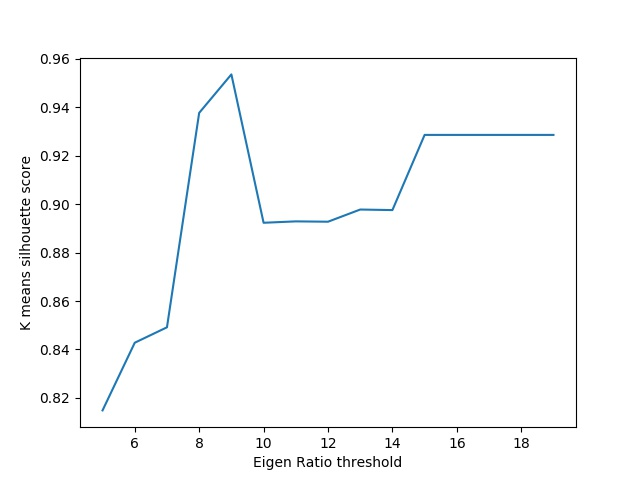
\includegraphics[width=0.8\linewidth]{threshold_vs_silhoutte_score.jpg}
		\caption{Plot of Silhoutte score vs eigenratio threshold}
		\label{sill}
	\end{figure}



	In order to arrive at the optimal value of $\tau$, we observe  the plot of the Silhoutte score of K-Means clustering, with $K=2$ (stochastic and non-stochastic), performed using the above feature set, as a function of the threshold value. The value of the threshold that results in the best Silhoutte clustering score is taken as $\tau$. This process is illustrated in the Silhoutte score plot shown in Fig\ref{sill}. For the time series considered here for illustration, it is evident from the plot that the best clustering is obtained at threshold value 9, resulting in the maximum value of Silhoutte score. Hence we use the corresponding $\tau = 9$ to arrive at the optimal hierarchical splitting and subsequent computing of the devised PCA-based features, VER and AUER.

	\subsection{Proof of Concept on Synthetic Data}
	The proposed approaches have been applied to standard synthetic signals. For stochastic class of signals, white noise and pink noise are considered; for non-stochastic class of signals, Lorenz system and Logistic map (for growth rate = 4) are considered.
	
	SVD-Decomposition based technique : The SVD decomposition of the data is computed, followed by the plot of the top two right singular vectors. This plot is utilized to determine the Betti descriptors. The plot in Fig. \ref{ele2_svd} corresponds to the E1 vs E2 plot for a realization of white noise, which is known to be stochastic. The plot shows one single blob implying Betti descriptor of (1 0), which has L1-norm of 1. As discussed before,  L1-norm of 1 implies that the timeseries is labelled as stochastic. On the other hand, the plot in Fig. \ref{ele2_svd_ns} corresponds to the E1 vs E2 plot of a realization of Lorentz system, which is known to be non-stochastic.  The plot shows two distinct voids, implying Betti descriptor to be (1 2), which has L1-norm of 3, implying that the timeseries is labelled as non-stochastic. This inference mechanism has been utilized on real data described in section \ref{rnd}.
	TODO Table with series name, betti descriptor, L1 norm, Label 
	\begin{figure}[ht]
		\centering
		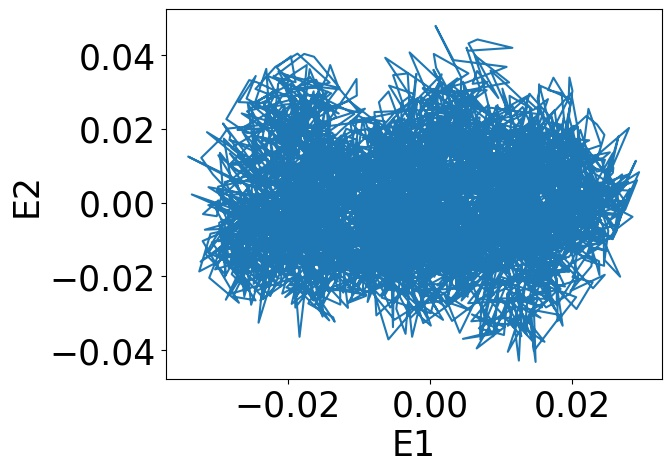
\includegraphics[width=0.8\linewidth]{svd_white_noise.jpg}
		\caption{Plot of Top-2 Right singular vectors for a stochastic timeseries}
		\label{ele2_svd}
	\end{figure}
	\begin{figure}[ht]
		\centering
		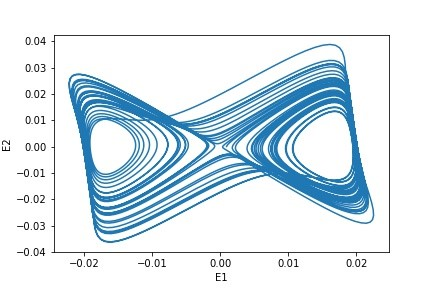
\includegraphics[width=0.8\linewidth]{svd_lorenz.JPG}
		\caption{Plot of Top-2 Right singular vectors for a non-stochastic timeseries}
		\label{ele2_svd_ns}
	\end{figure}
		PCA-Decomposition based technique :PCA-based features (i) VER and (ii) AUER  are computed for the considered synthetic signals which are 24 different realizations of white noise and logistic map (growth rate = 4). The scatter plot of these features for these realizations is shown Fig \ref{scatterplot} below. The plot makes it evident that in this feature space the two classes of timeseries, stochastic and non-stochastic, become linearly separable. Hence a linear SVM classifier is utilized. For training the SVM, computed features from white noise and Logistic map are utilized. For validating the trained SVM, 12 realizations of pink noise and Lorentz system are used. The classification on all 12 realizations of pink noise, yields the label stochastic, and the classification label for Lorentz system is obtained as non-stochastic, leading to perfect validation accuracy. This trained SVM is used to classify real data as described in section \ref{rnd}
	
	TODO Table with series name, PCA features, Label 
	\begin{figure}[h]
		\centering
		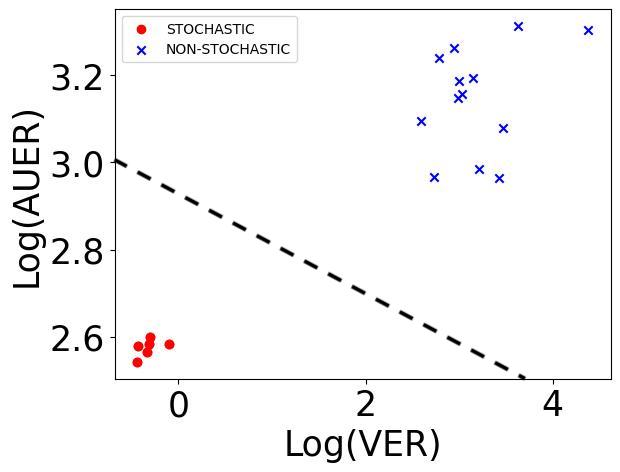
\includegraphics[width=0.8\linewidth]{Scatterplot_poc_variance_area_threshold_7.jpg}
		\caption{Scatter plot of PCA-based features for synthetic data}
		\label{scatterplot}
	\end{figure}
	
	
	%\begin{figure}[ht]
	%\centering
	%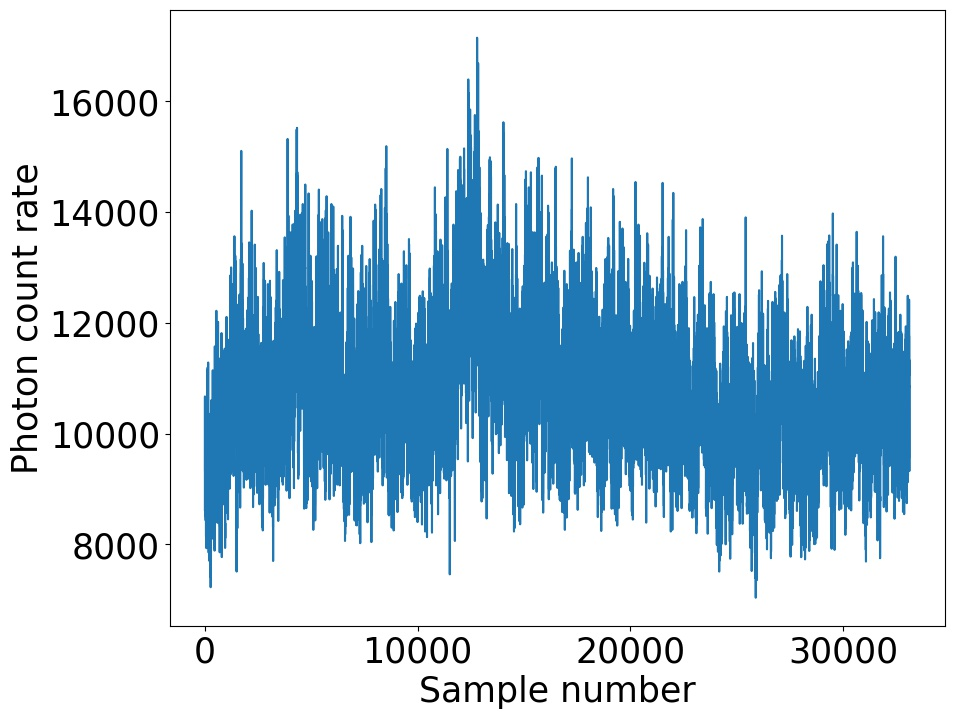
\includegraphics[width=0.8\linewidth]{sac_ascf_phi.jpg}
	%\caption{A representative stochastic time series of class $\phi$ of \textit{GRS 1915 + 105}. X-axis: Sample number (Scale: 0 - 35000), Y-axis: Photon count rate (Scale: 0 - 18000). }
	%\label{phi_ts}
	%\end{figure}
	%
	%\begin{figure}[ht]
	%\centering
	%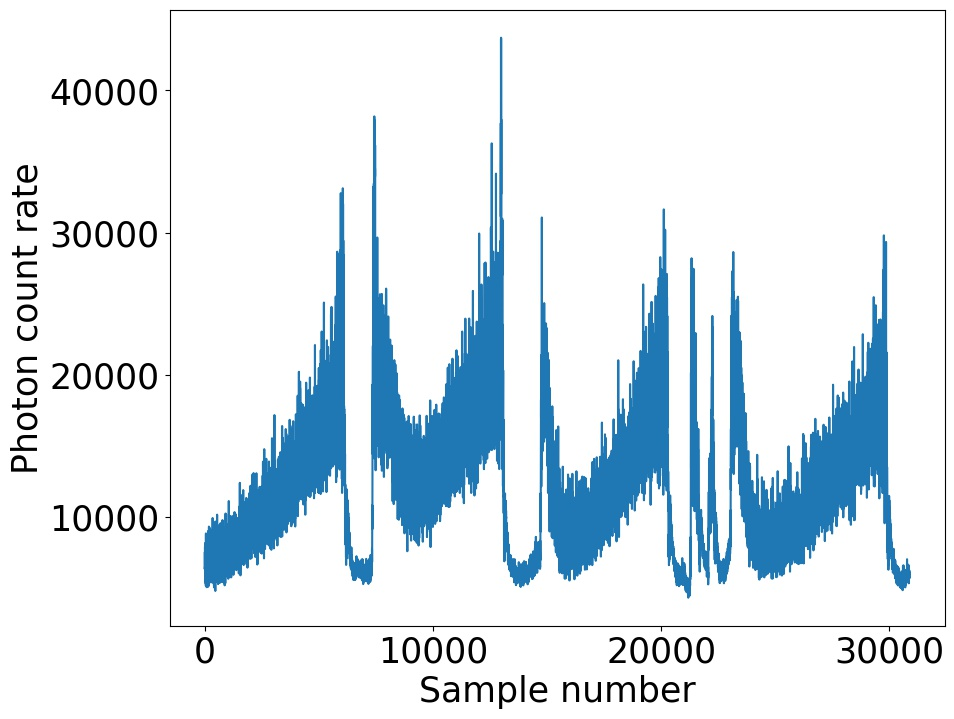
\includegraphics[width=0.8\linewidth]{sac_ascf_theta.jpg}
	%\caption{A representative non-stochastic time series of class $\theta$ of \textit{GRS 1915 + 105}. X-axis: Sample number (Scale: 0 - 35000), Y-axis: Photon count rate (Scale: 0 - 45000). }
	%\label{theta_ts}
	%\end{figure}
	
	\section{Results and Discussion} \label{rnd}
	In this section, we present the real data used, results obtained using proposed approaches and comparison with results in literature.
	
	\subsection{Real Data}
	The proposed approaches are illustrated on the publicly available data of \textit{GRS 1915 + 105} taken from website \cite{xte}. 12 distinct categories of time series are utilized from the available data. All these time series are re-sampled with a sampling interval of 0.1 second. These datasets  were  also used in the work reported in \cite{Adegoke2018}, where the authors use CI based approaches, leading us to be able to compare our obtained results with theirs.
	TODO..consistentently ..categories of time series in place of classes of time series
	TODO..Topological analysis ...Betti descriptors are used interchangebaly..we need to check
	\subsection{Results of SVD based analysis}
	
	%From SVD decomposition of the data matrix, we pick up the top 2 right singular vectors (E1, E2) corresponding to the temporal dynamics and plot E1 vs E2 for each time series. Figure \ref{svd_e1e2_nonstochastic} shows the panel of representative E1-E2 plots for time series  that are classified as non-stochastic and Figure \ref{svd_e1e2_stochastic}  shows the corresponding panels for time series that are classified as stochastic. The Betti number descriptors for each of the E1-E2 plots are tabulated in Table \ref{tab:results} under the column Betti descriptors. In order to infer the label of the time series from the Betti descriptors, We use the following strategy. Betti descriptor $\beta = (\beta_0, \beta_1)$. We use the L1-norm of $\beta$. If $\lvert \beta \rvert \gt 1$ then the time series is classified as non-stochastic else the time series is stochastic.
	
	From SVD decomposition of the data matrix, we plot the top 2 right singular vectors (E1 vs E2) to understand the temporal dynamics for each time series. Figure \ref{svd_e1e2_nonstochastic} shows representative E1 vs E2 plots for time series  that are classified as non-stochastic and Figure \ref{svd_e1e2_stochastic}  shows the corresponding plots for time series that are classified as stochastic. The Betti number descriptors for each of the E1 vs E2 plots are tabulated in Table \ref{tab:results} under the column \textit{Betti descriptor}. In order to infer the label of the time series from the Betti descriptors, we use the L1-norm of $\beta$, $\|\beta\|_1$. If $\|\beta\|_1 > 1$, the time series is classified as non-stochastic, else the time series is stochastic.
	
	
	%\begin{figure*}
	%  \centering
	%  \subfigure[]{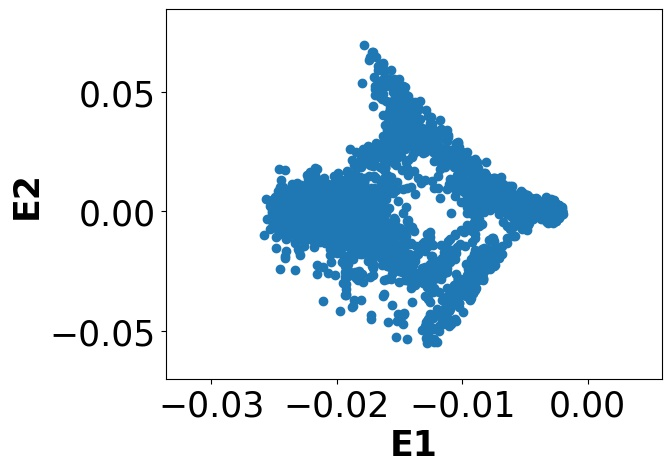
\includegraphics[width=0.25\textwidth]{images/sac_ascf_kappa_e1_vs_e2_m_2_tau_50.jpg}}
	%  \subfigure[]{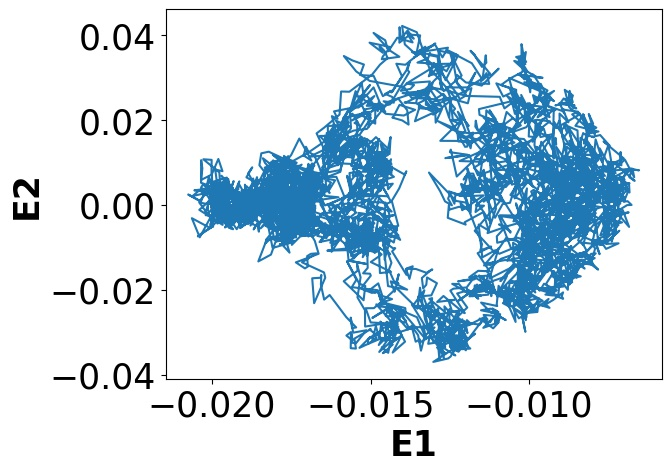
\includegraphics[width=0.25\textwidth]{images/sac_ascf_mu_e1_vs_e2_m_4_tau_80.jpg}}
	%  \subfigure[]{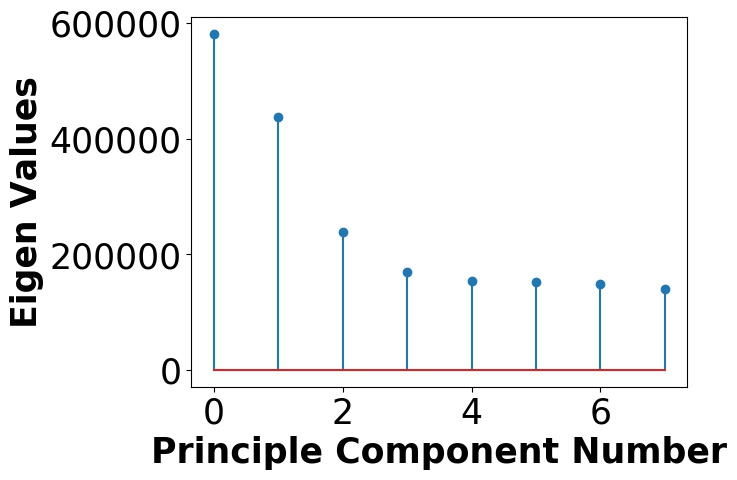
\includegraphics[width=0.25\textwidth]{images/sac_ascf_rho_e1_vs_e2_m_8_tau_20.jpg}}
	%  \caption{Plot of E1 vs E2 (top two right singular vectors) of data matrix for  representatives from non-stochastic time series of \textit{GRS 1915 + 105}. The series are $\kappa$, $\mu$ and $\rho$ from left to right.}
	%  \label{svd_e1e2_nonstochastic}
	%\end{figure*}
	
	
	%\begin{figure*}
	%  \centering
	%  \subfigure[]{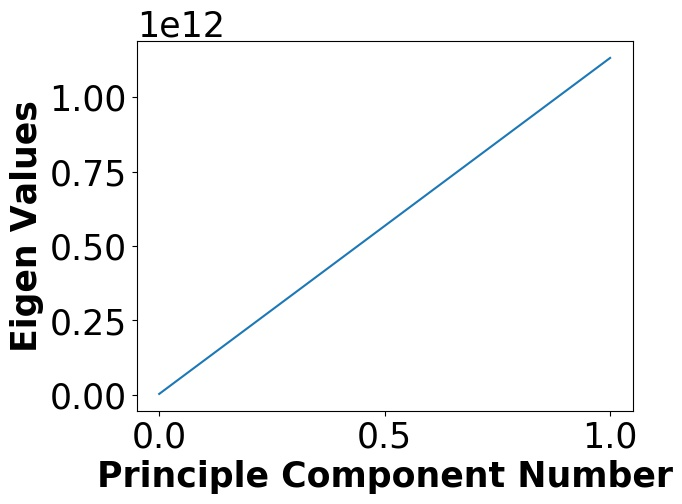
\includegraphics[width=0.25\textwidth]{images/sac_ascf_phi_e1_vs_e2_m_2_tau_20.jpg}}
	%  \subfigure[]{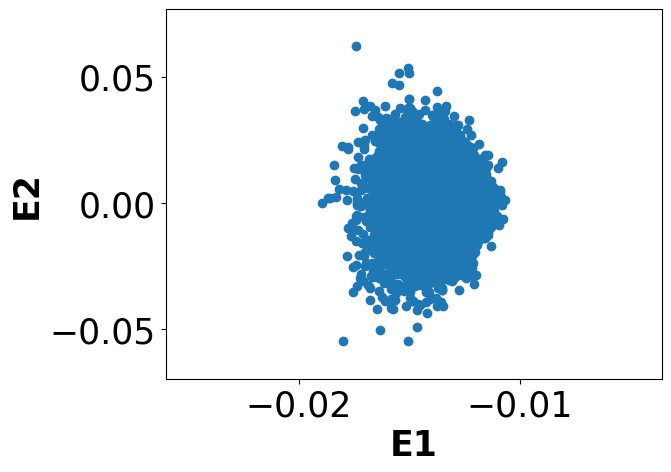
\includegraphics[width=0.25\textwidth]{images/sac_ascf_kai_e1_vs_e2_m_2_tau_20.jpg}}
	%  \subfigure[]{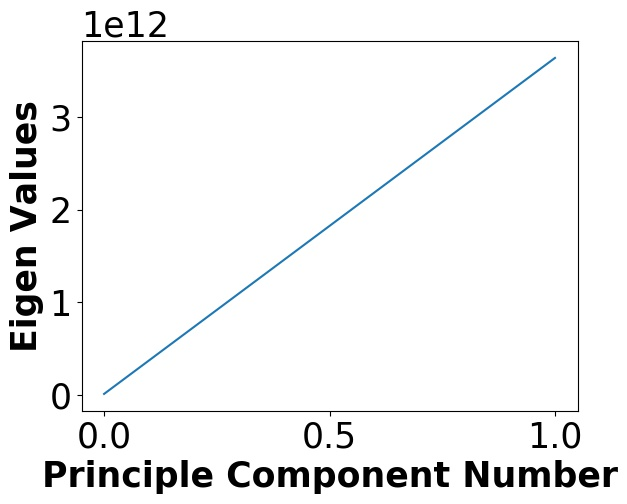
\includegraphics[width=0.25\textwidth]{images/sac_ascf_gamma_e1_vs_e2_m_2_tau_20.jpg}}
	%\caption{Plot of E1 vs E2 (top two right singular vectors) of data matrix for  representatives from  stochastic time series  of \textit{GRS 1915 + 105}. The series are $\phi$, $\chi$ and $\gamma$ from left to right.}
	%  \label{svd_e1e2_stochastic}
	%\end{figure*}
	
	TODO :Table of Betti number - Time series, Betti Descriptor, l1 norm , SVD label
	
	\subsection{Results of PCA based analysis}
	
	
	
	%\begin{figure}[ht]
	%\centering
	%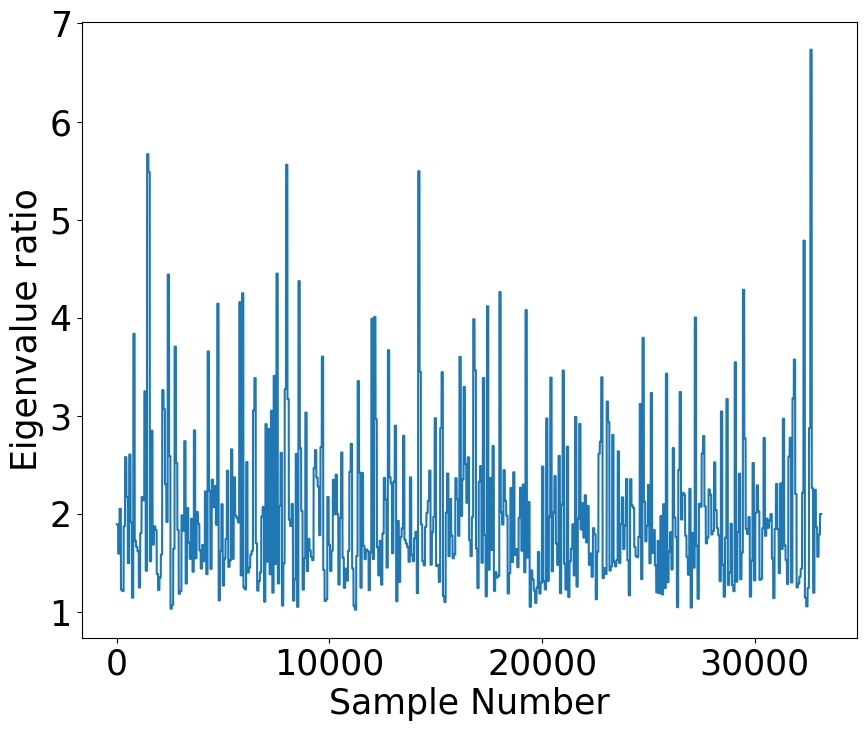
\includegraphics[width=0.8\linewidth]{sac_ascf_phi_eig.jpg}
	%\caption{Plot of eigenvalue ratio of the stochastic time series shown in Figure \ref{phi_ts}. X-axis: Sample number (Scale: 0 - 35000), Y-axis: Eigenvalue ratio (scale- 0 - 7). MER=7}
	%\label{phi_eig}
	%\end{figure}
	%
	%\begin{figure}[ht]
	%\centering
	%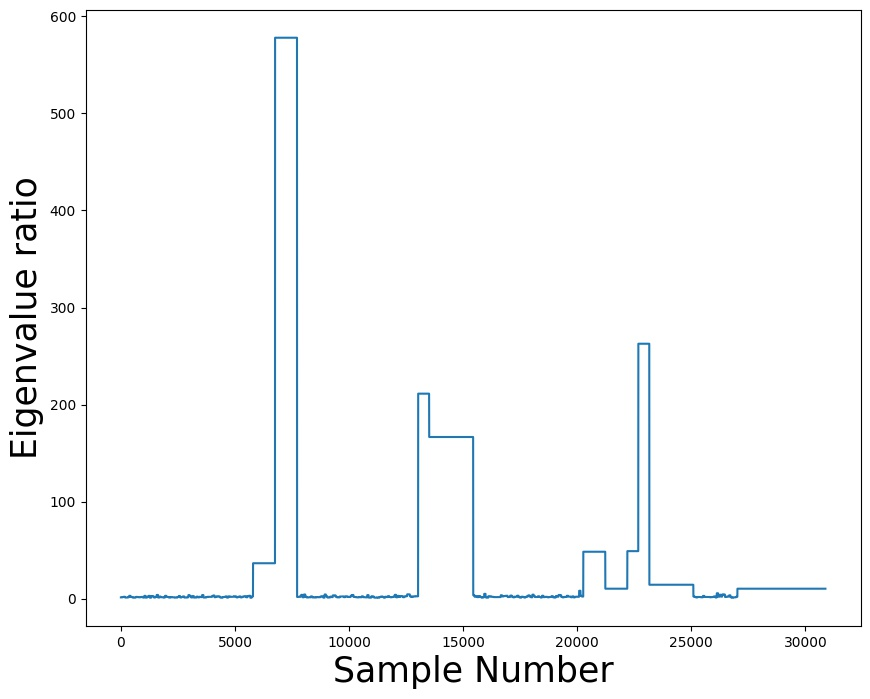
\includegraphics[width=0.8\linewidth]{sac_ascf_theta_eig.jpg}
	%\caption{Plot of eigenvalue ratio of the  non-stochastic time series shown in Figure \ref{theta_ts}. X-axis: Sample number (Scale: 0 - 35000), Y-axis: Eigenvalue ratio (scale- 0 - 600). MER=577 }
	%\label{theta_eig}
	%\end{figure}
	
	Figures \ref{phi_eig} and \ref{theta_eig} show the eigenvalue ratio plots for stochastic time series shown in Figure \ref{phi_ts} and  non-stochastic time series shown in Figure \ref{theta_ts} respectively. We compute PCA-derived features, VER and AUER. These features are input to the SVM classifier to obtain the class labels.  
	\begin{itemize}
		\item VER: For a stochastic signal since the variation in the eigenvalue ratios is typically small, the computed variance across the values is small. On the other hand, for a non-stochastic signal, since the eigenvalue ratios occupy diverse values, VER is typically high.
		\item AUER: For a stochastic time series, since the eigenvalue ratios  are small across the entire span, the value of AUER is also small. However, for a non-stochastic signal, the eigenvalue ratios remain high for longer time intervals. Hence the value of AUER is significantly higher.
	\end{itemize}
	
	\subsection{Consolidated Results}
	
	\subsubsection{ Comparison of Results}
	Table \ref{tab:results}  tabulates the computed features and the respective inferences using the proposed approaches. Comparison of our results with CI based approach \cite{Adegoke2018} is also presented. The columns of the table are described below.
	
	\begin{enumerate}
		\item Column 1 (\textit{Class}) gives the class of the time series \cite{Adegoke2018}.
		\item Column 2 (\textit{diskbb}) and column 3 (\textit{PL}) give quantities diskbb and  PL, respectively, which indicate the spectral states of the black hole \cite{Adegoke2018}.
		\item Column 4 (CI Inference) gives the inference about the state of the time series using CI approach \cite{Adegoke2018}.
		\item Column 5  SVD based inference.
		\item Our inference using these PCA features is given in column XX.
		\item Finally the last column gives if there is a match between all three inferences.
	\end{enumerate}
	
	
	\begin{table*}[t]
		\caption{Timeseries: Comparison between CI based label and inference using proposed approaches. The mismatched time series class, $\delta$, is shown in bold. (Here $NS$ stands for non-stochastic and $S$ stands for stochastic)}
		\begin{center}
			\begin{tabular}{|p{0.5cm}|p{0.75cm}|p{0.75cm}|p{0.75cm}|p{0.75cm}|p{1cm}|p{0.5cm}|p{0.75cm}|}
				\hline
				Class & CI \newline Label & Betti Norm & SVD \newline Label & VER & AUER & PCA \newline Label  &  Match \\
				\hline
				$\beta$ & NS & 4 & NS & 483 & 43 & NS & Yes\\
			\hline
				$\theta$  & NS &  5 & NS & 778 & 58 & NS  &  Yes \\
				\hline
			$\lambda$ & NS & 4 & NS & 6782 & 314 & NS & Yes \\
			\hline
				$\kappa$ & NS & 4 & NS & 5199 & 144 & NS & Yes \\
			\hline
		$\mu$ & NS & 2 & NS & 51 & 12 & NS & Yes \\
		\hline
			$\nu$ & NS & 7 & NS & 32 & 16 & NS & Yes \\
			\hline
$\alpha$ & NS & 6 & NS & 1.9 & 27.7 & NS & Yes \\
\hline
$\rho$ & NS & 2 & NS & 147 & 35 & NS & Yes \\
\hline
$\delta$ & S & 1 & S & 9.7 & 26.2 & NS & NO \\
\hline
$\phi$ & S & 1 & S & 0.5 & 15 & S & YES \\
\hline
$\gamma$ & S & 1 & S & 1 & 16 & S & YES \\
\hline
$\chi$ & S & 1 & S & 0.25 & 6.05 & S & YES \\
\hline
%				\textbf{$\delta$}  & \textbf{48} & \textbf{50} &  \textbf{S} & \textbf{(1,0)}& \textbf{Stochastic}& \textbf{42} & \textbf{9.74} & \textbf{26.2} & \textbf{Non-stochastic} &  \textbf{No} \\
%				\hline
%				$\phi$  & 50 & 34 & S & (1,0)& Stochastic & 7 & 0.5 & 15 & Stochastic &  Yes \\
%				\hline
%				$\gamma$  & 60 & 31 & S & (1,0)& Stochastic & 12 & 1 & 16 & stochastic &  Yes \\
%				\hline
%				$\chi$  & 09 & 89 & S & (1,0)& Stochastic & 5.6 & 0.25 & 6.05 & Stochastic &  Yes \\
			%	\hline
			\end{tabular}
			\label{tab:results}
		\end{center}
	\end{table*}
	


		\begin{table*}[t]
		\caption{Blackhole state Inference Comparison across CI-based and proposed approaches:}
		\begin{center}
			\begin{tabular}{|p{0.5cm}|p{0.8cm}|p{0.75cm}|p{1.25cm}|p{1.25cm}|p{1.25cm}|p{0.70cm}|}
				\hline
				Name & diskbb & PL & State by CI & State by SVD  & State by PCA  &  Match \\
				\hline
				$\beta$ & 46 & 52 & ADAF & ADAF & ADAF & Yes\\
				\hline
                $\theta$ & 11 & 88 & ADAF & ADAF & ADAF & Yes\\
				\hline
                $\lambda$ & 54 & 46 & Keplerian & Keplerian & Keplerian & Yes\\
				\hline
               $\kappa$ & 59 & 51 & Keplerian & Keplerian & Keplerian & Yes\\
				\hline
               $\mu$ & 56 & 41 & Keplerian & Keplerian & Keplerian & Yes\\
               \hline
              $\nu$ & 28 & 72 &  ADAF & ADAF & ADAF & Yes\\
              \hline
             $\alpha$ & 23 & 77 &  ADAF & ADAF & ADAF & Yes\\
             \hline
             $\rho$ & 28 & 72 &  ADAF & ADAF & ADAF & Yes\\
\hline
 $\delta$ & 48 & 50 & ADAF & ADAF & GAAF & NO\\
\hline
$\phi$ & 50 & 34 & slimdisc & slimdisc & slimdisc & YES\\
\hline
$\gamma$ & 60 & 31 & slimdisc & slimdisc & slimdisc & YES\\
\hline
$\chi$ & 09 & 89 & GAAF & GAAF & GAAF & YES\\
\hline
%				$\chi$  & 09 & 89 & S & (1,0)& Stochastic & 5.6 & 0.25 & 6.05 & Stochastic &  Yes \\
				\hline
			\end{tabular}
			\label{tab:results}
		\end{center}
	\end{table*}
	
	%\begin{figure}
	% \centering
	% 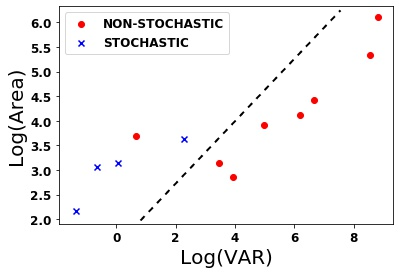
\includegraphics[width=.8\linewidth]{variance_area.drawio.png}
	% \caption{Feature space (VAR and Area) shows that the two classes are well separated. The dashed line shows the decision boundary separating the two classes. The label of one of the time series is ambiguous.}
	% \label{fig:variance_area_fs}
	%\end{figure}
	\subsection{Identification of black hole states}
	
	We observe that SVD based analysis results in classification are consistent with CI based results for all the 12 categories of time series. However, with the PCA based approach the inference for  $\delta$ time series is not consistent with the other two approaches. We observe that the PCA based features, VER and AUER, make the space of timeseries, linearly separable, as shown in Figure \ref{fig:variance_area_fs}. This feature space is utilized to train a linear SVM. According to the CI based analysis $\delta$ turns out to be in between states slim disc and GAAF \cite{Adegoke2018}. However, the present analysis shows that $\delta$ falls in between ADAF and Keplerian disc.
	
	
	\section{Conclusion}
	Exploring different techniques in order to have a conclusive inference for black hole systems turns out to be indispensable. We explore two different classical matrix based techniques to identify states of \textit{GRS 1915+105} black hole using the time series obtained from \textit{RXTE} satellite data. Based on our analysis, we are able to identify two extreme temporal dynamical classes of accretion around black holes. In the first approach we extend  SVD decomposition to understand temporal dynamics,  by adding  topological descriptors, to classify time series as stochastic vs non-stochastic. In yet another approach, a novel application of  PCA  to characterize the time series is proposed. We compare inferences of the CI based approach with those obtained using the proposed matrix based methods. Of the 12 categories of time series analysed, a mismatch is observed in the PCA based inference of only one class, while all other classes concur.
	
	
	%Several real-world phenomena are studied by collecting associated measurements over time, popularly called as timeseries. Understanding the phenomenon, typically begins by determining if the timeseries is stochastic (noise-like) or non-stochastic (which has a well-defined structure). Stochastic timeseries may be seen as noise, while non-stochastic timeseries could reveal more about the associated physcial phenomenon. This problem of stochastic vs non-stochastic classification runs across domains such as weather, finance, agriculture, astronomy, etc.  For a specific problem in astronomy, in the context of data obtained from the RXTE satellite, the problem of stochastic vs non-stochastic classification can help in identifying states of the black hole, \textit{GRS 1915 + 105}. The most-popular method for stochastic vs non-stochastic classification follows Correlation Integral (CI) based approach, which is computationally expensive. In this study, we propose two computationally simple matrix-based approaches, for classifying a timeseries as stochastic or non-stochastic, which are : (a) SVD-based technique followed by topological analysis (b) PCA-based technique. The proposed methods have been applied to 12 categories of timeseries pertaining to blackhole \textit{GRS 1915 + 105}, obtained from RXTE satellite. Comparisons of obtained results with those in literature are also presented. The order of computational complexity using the proposed approaches is reduced by a factor of TOBEDONExxxxTOBEDONE, as compared to the current gold-standard CI-based approach. It is found that among the proposed matrix based methods, SVD analysis concurs with CI based analysis on all 12 categories of time series utilized. However, the inference using PCA based approach illustrates that one class among the 12 turns out to be inconsistent with the other approaches. Investigation into these (in)consistencies  is expected to have long standing implications in astrophysics and otherwise.
	
	% Ref from Signal Processing Letters Dispersion Entropy: A Measure for Time-Series
	%Analysis
	%Mostafa Rostaghi and Hamed Azami
	
	
\end{document}



